% !TEX root = ../notes_missingsemester.tex
% Chapter 7: Face the World — Frontend & Nginx
%%%%%%%%%%%%%%%%%%%%%%%%%%%%%%%%%%%%%%%%%%%%%%%%%%%%%%%%%%%%%%%%%%%%%%

\index{Nginx}\index{reverse proxy}\index{frontend}\index{HTTPS}\index{HTTP}\index{TLS}\index{CORS}\index{JavaScript}\index{HTML}\index{CSS}\index{canvas}
\chapter{Reverse Proxy \& Frontend}
\printchapterversion{07_frontend_nginx}
\newthought{Form follows function}

% ==============================================================================================
% BLOCK 1: INTRODUCTION
% ==============================================================================================

\section{The Why}\index{HTTP}\index{Nginx}\index{reverse proxy}

\newthought{The only way in today} is a \texttt{curl} one-liner on
port 8000 with a secret header attached.
There is no human-friendly interface.
The backend is the engine of the service; the frontend is what builds an
experience around it and makes it accessible to people.
Engineers tend to undervalue the frontend, and pay for it by not being
understood.

\newthought{This block} closes that gap.
We put Nginx\index{Nginx} in front of \texttt{uvicorn}\index{uvicorn},
serve a small static frontend out of \texttt{/var/www/pixelwise/},
move the public surface off the application's port 8000 onto the standard
web port 80, and route browser traffic through the same
\texttt{POST /classify} and \texttt{GET /results} handlers we wired up in
Block~6.


\begin{figure}
\centering
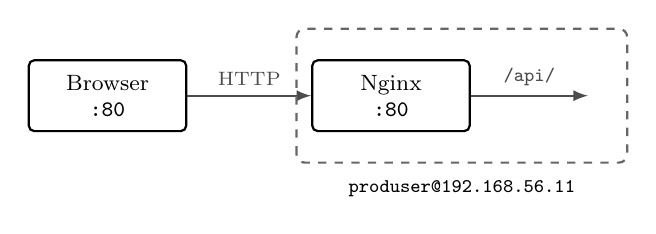
\begin{tikzpicture}[
    every node/.style={font=\footnotesize, align=center},
    box/.style={rectangle, draw=black, thick, rounded corners=2pt, minimum width=2.0cm, minimum height=0.9cm, inner sep=4pt},
    arr/.style={-latex, thick, black!70}
]
\node[box] (br) at (-1.2, 0) {Browser\\\texttt{:80}};
\node[box] (ng) at (2.4, 0)  {Nginx\\\texttt{:80}};
\draw[arr] (br.east) -- node[above]{\scriptsize HTTP} (ng.west);
\draw[arr] (ng.east) -- node[above]{\scriptsize \texttt{/api/}} (4.9, 0);
\draw[black!60, thick, dashed, rounded corners=3pt]
    (1.2, -0.85) rectangle (5.4, 0.85);
\node[font=\scriptsize, anchor=north] at (3.3, -0.95)
    {\texttt{produser@192.168.56.11}};
\end{tikzpicture}
\caption{\rule{0pt}{1.4cm}\\
The browser reaches our reverse proxy Nginx over HTTP on port 80. Nginx serves the static
frontend and forwards \texttt{/api/} requests inward to the Block~6 service
on \texttt{localhost:8000}. The dashed box is the \texttt{prod} VM, where
only Nginx faces the network. The optional HTTPS exercise upgrades the
browser connection to TLS on port 443.}
\label{fig:reverse_proxy_flow}
\end{figure}



\newthought{Why not expose \texttt{uvicorn} to the internet directly?}
Put the process that classifies digits on the public network and every
malformed request, port scan, and slow-connection flood hits your
application code, where one crash takes the whole site down.
A reverse proxy sits in front instead: It accepts each request, calls
\texttt{uvicorn} on port 8000 itself, and returns the response, so the
client never touches the application.
Nginx absorbs the rough traffic at the edge and forwards only clean
requests inward, and we can restart, scale, or swap the upstream without
the public URL ever moving.

\subsection{Hands On Experience}

\newthought{The product is invisible} until you give it a front door.
From here on, renting a cheap server is the only step between your project
and the world.
The gap between a codebase on your laptop and a live service on the
internet is huge.
Build, share, learn, and have fun, and do not let anyone make your world
small and narrow.


\newthought{This seventh block}\index{PixelWise} introduces the public
surface for PixelWise.
By the end you will have
\begin{itemize}
    \item installed and configured Nginx as a reverse proxy on \texttt{prod},
    \item served a static HTML and JavaScript drawing frontend from \texttt{/var/www/pixelwise/},
    \item and reached the live application in a browser.
\end{itemize}
An optional section at the end of the block carries the edge further,
terminating TLS so the site answers on \texttt{https://}.



% ==============================================================================================
\newpage
\section{Optional Exercise: Catch Up to \texttt{v0.5}}\index{exercises}\index{Git!tag}\index{recovery}

\marginnote{\newthought{Tag map.}\index{Git!tag}
\texttt{v0.5} marks the end of Block~6, \texttt{v0.6} will mark the end
of this block.
Browse the full set at
\url{https://github.com/schutera/pixelwise/tags}.}

\newthought{Catching up via tag.}\index{Git!tag}\index{recovery}
If you are not already at the end of Block~6, rewind both VMs to
\texttt{v0.5}: PostgreSQL provisioned, the \texttt{pixelwise} role and
database created, the SQLAlchemy \texttt{Prediction} model wired into
the FastAPI handlers, and \texttt{POST /classify} writing rows that
\texttt{GET /results} reads back. Both VMs follow the same sequence;
run \texttt{dev} first, then \texttt{prod}.

\marginnote{\newthought{Sequence on \texttt{dev}.}\\[0.4em]
\texttt{cd \textasciitilde/pixelwise}\\
\texttt{git fetch origin -{}-tags}\\
\texttt{git reset -{}-hard v0.5}\\
\texttt{cp .env.example .env}\\
\texttt{nano .env}\\
\texttt{source .venv/bin/activate}\\
\texttt{pip install -r requirements.txt}\\
\texttt{bash setup-server.sh}\\
\texttt{python init\_db.py}\\[0.3em]
Set \texttt{DB\_PASSWORD} in \texttt{.env} and keep the
\texttt{SECRET\_API\_KEY} from Block~5. If \texttt{.venv/} is missing,
run \texttt{python3 -m venv .venv} first.}

\newthought{On \texttt{dev}.} Run the margin sequence.
\texttt{setup-server.sh} installs PostgreSQL and provisions the
\texttt{pixelwise} role and database; \texttt{python init\_db.py}
creates the \texttt{predictions} table.

\marginnote{\newthought{Sequence on \texttt{prod}.}\\[0.4em]
\texttt{ssh produser@192.168.56.11}\\
\texttt{cd /opt/pixelwise}\\
\texttt{git fetch origin -{}-tags}\\
\texttt{git reset -{}-hard v0.5}\\
\texttt{cp .env.example .env}\\
\texttt{nano .env}\\
\texttt{source .venv/bin/activate}\\
\texttt{pip install -r requirements.txt}\\
\texttt{bash setup-server.sh}\\
\texttt{python init\_db.py}\\[0.3em]
Use the same \texttt{DB\_PASSWORD} as on \texttt{dev}.}

\newthought{On \texttt{prod}.} Same sequence after the \texttt{ssh} and
\texttt{cd}. Verify from \texttt{dev}:
\texttt{curl -s http://192.168.56.11:8000/results} should return
\texttt{\{"results":[]\}}. Both machines are now at the end-of-Block~6
state, ready for Block~7.

% ==============================================================================================
% BLOCK 2: CONCEPTS AND PRACTICE
% ==============================================================================================

\newpage
\section{Reverse Proxies and Nginx}\index{Nginx}\index{reverse proxy}

\newthought{A reverse proxy sits at the edge.}\index{reverse proxy}
The client opens a connection to the proxy, the proxy opens a connection
to the upstream, and the response flows back along the same path.


\newthought{Forward versus reverse.}\index{proxy}
A forward proxy sits in front of the client and reaches out to many
servers on the client's behalf, the way a corporate web filter does.
A reverse proxy sits in front of the server and serves many clients on
the server's behalf.
Same word, opposite direction.

\newthought{Nginx} is the reverse proxy this course uses.
\marginnote{Nginx\index{Nginx}:\\
\url{https://nginx.org/}\\
Nginx documentation:\\
\url{https://nginx.org/en/docs/}}

It is fast, well documented, and the most common piece of software you
will find sitting in front of Python and Node services in production.
The configuration is a tree of nested blocks: A top-level \texttt{http}
context, \texttt{server} blocks inside it, and \texttt{location} blocks
inside each \texttt{server}.
Each \texttt{server} block declares a listen port and a hostname; each
\texttt{location} declares how to handle requests whose paths match a
pattern.

\newthought{Three roles in one process.}
In the PixelWise stack Nginx wears three hats at once:
\begin{itemize}
    \item As a static file server, it ships HTML, CSS, and JavaScript
    from \texttt{/var/www/pixelwise/} to the browser as fast as the
    kernel can read them.
    \item As a reverse proxy, it forwards every request whose path
    begins with \texttt{/api/} to \texttt{uvicorn} on
    \texttt{localhost:8000}.
    \item As a TLS terminator, it holds the certificate and the private
    key, so the public connection is encrypted while the internal
    connection to \texttt{uvicorn} stays plain HTTP.
\end{itemize}

\marginnote{\newthought{Why a high port?}\index{ports}
On Linux, ports below 1024 are privileged; binding requires either root
or a capability granted by root.
\texttt{uvicorn} runs as the unprivileged \texttt{produser}, so it
listens on port 8000 where no special permission is needed.
Nginx is started by \texttt{systemd} as root, binds 80 and 443, then
drops its worker processes to an unprivileged user.}


\newthought{\texttt{nginx -t}} is the cheapest debugging tool in the
chapter.
It parses the configuration without applying it, prints \texttt{syntax
is ok} when the file is well formed, and points at the line and column
of the first problem when it is not.
Run it before every \texttt{systemctl reload nginx} and the daemon will
never refuse to start because of a missing semicolon or a typo in a
directive name.







% ==============================================================================================
\newpage
\section{Exercise: Install Nginx and the First Proxy Pass}\index{exercises}\index{Nginx}

\newthought{Install Nginx on \texttt{prod}.}
On a fresh \texttt{prod} VM, install the package and confirm the daemon
is up and listening on port 80:

\begin{verbatim}
ssh produser@192.168.56.11
sudo apt update
sudo apt install -y nginx
systemctl status nginx --no-pager
\end{verbatim}

\marginnote{\newthought{The default site.}\index{Nginx}
A fresh install ships an Nginx \texttt{Welcome} page from
\texttt{/etc/nginx/sites-enabled/default}.
We will leave it in place until our own site is ready, then disable it
in one step so there is no confusion about which configuration is
serving requests.}

The first three lines should report \texttt{Active: active (running)}.
Visit \texttt{http://192.168.56.11} from your host browser; the default
Nginx welcome page proves the daemon is reachable on port 80 of the VM
over the host-only network.

\newthought{Author the site configuration on \texttt{dev}.}
The Nginx configuration is part of how the application runs, so it
belongs next to the code, the systemd unit, and the setup script.
Open the new file at \texttt{deploy/pixelwise.nginx} in the repository
on \texttt{dev}:

\begin{verbatim}
cd ~/pixelwise
nano deploy/pixelwise.nginx
\end{verbatim}

The file below is the first cut, plain HTTP on port 80, the frontend
served from disk, every request under \texttt{/api/} forwarded to
\texttt{uvicorn}:

\begin{verbatim}
# deploy/pixelwise.nginx
server {
    listen 80;
    server_name 192.168.56.11;

    # Serve the static frontend
    location / {
        root /var/www/pixelwise;
        index index.html;
        try_files $uri $uri/ =404;
    }

    # Forward API calls to uvicorn
    location /api/ {
        proxy_pass http://127.0.0.1:8000/;
        proxy_set_header Host $host;
        proxy_set_header X-Real-IP $remote_addr;
        proxy_set_header X-Forwarded-For $proxy_add_x_forwarded_for;
        proxy_set_header X-Forwarded-Proto $scheme;
    }
}
\end{verbatim}

\marginnote{\newthought{Trailing slash matters.}\index{proxy\_pass}
\texttt{proxy\_pass http://127.0.0.1:8000/} strips the matched
\texttt{/api/} prefix before forwarding.
Without the trailing slash, \texttt{/api/classify} would reach
\texttt{uvicorn} as \texttt{/api/classify} and FastAPI would answer
\texttt{404} because the route is registered as \texttt{/classify}.
One character, opposite outcomes.}

\marginnote{\newthought{\texttt{try\_files} is the static fallback.}\index{try\_files}
For a single-page frontend like ours, the directive tries the requested
path, then a directory listing, then returns \texttt{404}.
A more elaborate frontend with client-side routing would fall back to
\texttt{index.html} instead so deep links survive a reload.
Our app has one page, so the \texttt{404} fallback is correct.}

\newthought{Commit on \texttt{dev}, pull on \texttt{prod}.}
The configuration belongs in the repository so a fresh VM can pick it up
from a clean clone instead of from somebody's terminal history:

\begin{verbatim}
cd ~/pixelwise
git add deploy/pixelwise.nginx
git commit -m "Add Nginx reverse proxy config"
git push
\end{verbatim}

Then on \texttt{prod}, pull the file into place:

\begin{verbatim}
ssh produser@192.168.56.11
cd /opt/pixelwise
git pull
\end{verbatim}

\newthought{Install the site on \texttt{prod}.}
Nginx looks for active sites under \texttt{/etc/nginx/sites-enabled/}.
The conventional pattern is to keep the real files under
\texttt{sites-available/} and symlink the active ones into
\texttt{sites-enabled/}, so disabling a site is one \texttt{rm} away:

\begin{verbatim}
sudo cp deploy/pixelwise.nginx \
    /etc/nginx/sites-available/pixelwise
sudo ln -sf /etc/nginx/sites-available/pixelwise \
    /etc/nginx/sites-enabled/pixelwise
sudo rm -f /etc/nginx/sites-enabled/default
sudo nginx -t
sudo systemctl reload nginx
\end{verbatim}

\marginnote{\newthought{Reload, not restart.}\index{Nginx}
\texttt{systemctl reload nginx} tells the master process to re-read the
configuration and gracefully replace its workers without dropping any
in-flight connection.
\texttt{restart} would kill the master and start it again, briefly
closing the listening sockets.
Reload is the default for configuration changes; restart is for the rare
case where reload is not enough.}

\newthought{Create the frontend directory.}
The \texttt{location /} block points at \texttt{/var/www/pixelwise/}
as the document root.
That directory does not exist yet on \texttt{prod}, and the next
exercise will fill it.
For now, drop a placeholder so the proxy pass has something to serve
when the path is \texttt{/}:

\begin{verbatim}
sudo mkdir -p /var/www/pixelwise
echo "PixelWise frontend stub" | \
    sudo tee /var/www/pixelwise/index.html
\end{verbatim}

\newthought{Did the proxy take?}\index{verification}
From \texttt{dev}, hit the proxied API and the static path back to back:

\begin{verbatim}
curl -s http://192.168.56.11/
curl -s http://192.168.56.11/api/health
\end{verbatim}

\marginnote{\newthought{Did it take on \texttt{prod}?}\index{verification}
\texttt{curl -s http://192.168.56.11/} should print the placeholder text.
\texttt{curl -s http://192.168.56.11/api/health} should print
\texttt{\{"status":"ok","model\_version":"v1"\}}.
The first answer came from Nginx reading a file on disk; the second
travelled from Nginx to \texttt{uvicorn} on port 8000 and back.
The browser sees one origin, \texttt{http://192.168.56.11}, even though
two very different processes produced the two responses.}

The first line should print \texttt{PixelWise frontend stub}.
The second should print the same JSON \texttt{uvicorn} would have given
you on port 8000, except now Nginx is the one that took the request.
Two different programs answered two paths, and from the outside they
look like one service on one port.







% ==============================================================================================
\newpage
\section{The Static Frontend}\index{frontend}\index{HTML}\index{JavaScript}\index{canvas}

\newthought{HTML for structure, CSS for layout, JavaScript for
behaviour.}\index{HTML}\index{CSS}\index{JavaScript}
Those are the three pieces a browser needs to render an interactive page,
and the three files PixelWise ships.
\begin{itemize}
    \item HyperText Markup Language, HTML, describes the document tree.
    \item Cascading Style Sheets, CSS, describe how it looks.
    \item JavaScript, JS, describes what happens when the user clicks,
    draws, or types.
\end{itemize}
The browser is the runtime, the network is the transport, and the server
is a file system that happens to speak HTTP.

\marginnote{\newthought{Why no framework?}\index{frontend}
React, Vue, and Svelte solve problems that show up at scale: Component
reuse across dozens of views, state management across complex
interactions, routing across many pages.
PixelWise has one page, one canvas, one results panel.
A framework would add a Node.js toolchain, a bundler, a learning curve
orthogonal to this course, and an extra layer hiding the bytes that
actually travel between browser and server.
Vanilla JS keeps the HTTP layer visible.}

\newthought{The page is a single canvas, two buttons, and a results panel.}
The drawing area is a \texttt{<canvas>} element shown at 280 by 280
pixels, a tenfold magnification of the 28 by 28 grid the model actually
reads.
The JavaScript paints straight into that grid, so the user draws at the
model's own resolution and watches the strokes pixelate as they land.
A \texttt{Classify} button extracts the pixel array and posts it.
A results panel renders the predicted digit, the confidence, and a
scrolling history pulled from \texttt{GET /api/results}.
That is the whole user surface.

\newthought{The \texttt{fetch} call} is the bridge between the browser
and the backend.\index{fetch}
\texttt{fetch} is the browser's modern HTTP client, a Promise-based
function that takes a URL and an options object and returns a response
the JavaScript can read as JSON, text, or bytes.
A \texttt{POST} to \texttt{/api/classify} carries the pixel array in
the body and the API key in a header, and waits for the JSON answer.
The exercise below builds this into \texttt{app.js}, where the
\texttt{classify} function issues exactly this request.

\marginnote{\newthought{Same-origin by design.}\index{same-origin}
The page is served from \texttt{http://192.168.56.11/} and posts to
\texttt{/api/classify} on the same host.
The browser treats both as the same origin because the scheme, host, and
port all match.}

\marginnote{\newthought{Open by design.}\index{API!authentication}\index{X-API-Key}
The \texttt{X-API-Key} header sits on \texttt{POST /api/classify}
because that endpoint is gated.
\texttt{GET /api/results} and \texttt{GET /api/health} carry no header
because they are unprotected: The browser renders the results panel and
probes the service without juggling a secret in client-side JavaScript.
That is acceptable for the demo here; in a real product
\texttt{/api/results} would move behind a session cookie or a short-lived
token from a proper login flow.}

\newthought{The relative path is the headline.}\index{URL design}
\texttt{fetch("/api/classify", \dots)} names no hostname or port.
It resolves against the URL the page was loaded from, so the same
JavaScript runs unchanged in the classroom on
\texttt{http://192.168.56.11} and in production on
\texttt{https://pixelwise.yourdomain.com}.
The frontend has no knowledge of where the backend lives, because the
backend lives wherever the frontend was served from.

% ==============================================================================================
\newpage
\section{Exercise: Build and Deploy the Frontend}\index{exercises}\index{frontend}

\newthought{Create the frontend directory on \texttt{dev}.}
The three files live in the repository under \texttt{frontend/} so they
travel with the code, get reviewed in pull requests, and reach
\texttt{prod} through the same Git path as the Python:

\begin{verbatim}
cd ~/pixelwise
mkdir -p frontend
nano frontend/index.html
\end{verbatim}

The HTML is small.
One canvas, two buttons, a result line, a recent-predictions list, one
stylesheet link, and one script tag at the bottom so the document tree is
built before the JavaScript looks for elements in it:

\begin{verbatim}
<!doctype html>
<html lang="en">
<head>
    <meta charset="utf-8">
    <meta name="viewport"
        content="width=device-width, initial-scale=1">
    <title>PixelWise</title>
    <link rel="stylesheet" href="style.css">
</head>
<body>
    <h1>PixelWise</h1>
    <p>Draw a digit, then click Classify.</p>
    <canvas id="pad" width="280" height="280"></canvas>
    <div class="controls">
        <button id="classify">Classify</button>
        <button id="clear">Clear</button>
    </div>
    <div id="result"></div>
    <h2>Recent predictions</h2>
    <ul id="history"></ul>
    <script src="app.js"></script>
</body>
</html>
\end{verbatim}

\marginnote{\newthought{Why a 280-pixel canvas?}\index{canvas}
The model expects 28 by 28 grayscale pixels.
Drawing at that size on a modern display would feel like trying to write
on a postage stamp.
So the visible canvas is that 28 by 28 grid magnified ten times: The user
gets a comfortable pad, the model gets the input shape it was trained on,
and nothing is hidden, because the chunky blocks on screen are exactly the
pixels that travel to the API.}

\newthought{Author the stylesheet} next to the HTML.
The styling is minimal: A centred column, a visible canvas border, a
button row, a result line, and a monospace history list.
The point is readability, not visual design:

\begin{verbatim}
nano frontend/style.css
\end{verbatim}

\begin{verbatim}
body {
    font-family: system-ui, sans-serif;
    max-width: 480px;
    margin: 2rem auto;
    padding: 0 1rem;
}
canvas {
    border: 1px solid #333;
    background: #fff;
    touch-action: none;
    display: block;
}
.controls { margin: 0.5rem 0 1rem 0; }
button {
    padding: 0.5rem 1rem;
    margin-right: 0.5rem;
    font-size: 1rem;
}
#result {
    font-size: 1.25rem;
    min-height: 1.5rem;
    margin-bottom: 1rem;
}
#history li { font-family: monospace; }
\end{verbatim}

\newthought{Author the script.}\index{JavaScript}
\texttt{frontend/app.js} wires the canvas to the mouse, builds the pixel
array, posts it, renders the prediction, and refreshes the history list.
Open the file:

\begin{marginfigure}
    \centering
    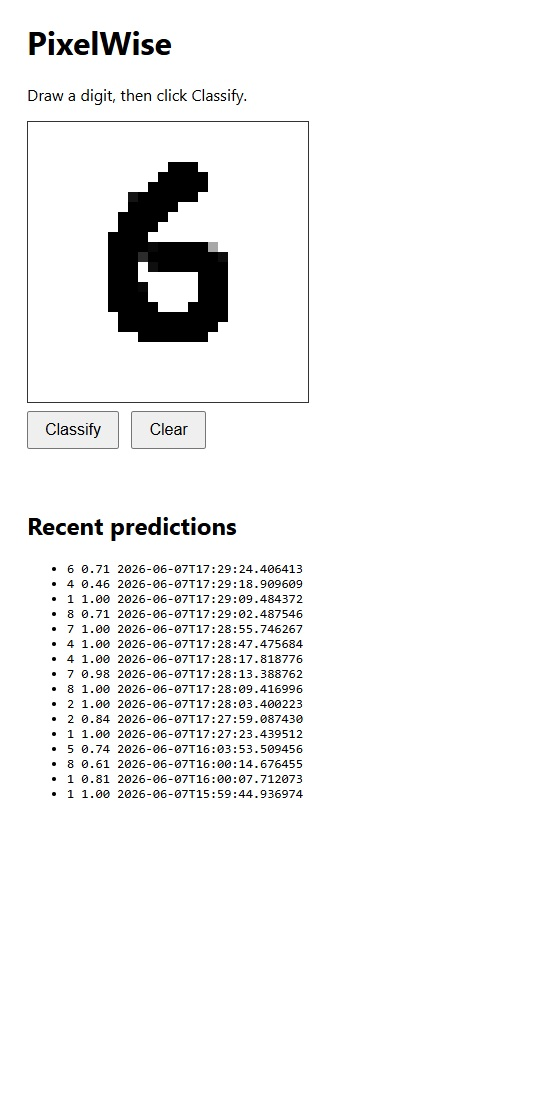
\includegraphics[width=\marginparwidth]{./figures/pixelwise_frontend.jpg}
    \caption{The finished frontend in the browser: The canvas, the
    \texttt{Classify} and \texttt{Clear} buttons, the result line, and the
    recent-predictions list. Nginx serves these files and forwards the
    \texttt{/api/} calls to FastAPI on \texttt{localhost:8000}.}
    \label{fig:pixelwise_frontend}
\end{marginfigure}

\begin{verbatim}
nano frontend/app.js
\end{verbatim}

\begin{verbatim}
// frontend/app.js
const API_KEY = "REPLACE_ME";  // overwritten on deploy

const N = 28;       // the model's input grid
const SCALE = 10;   // on-screen pixels per grid cell (280 / 28)

const pad = document.getElementById("pad");
const view = pad.getContext("2d");
view.imageSmoothingEnabled = false;  // draw crisp blocks

// The real drawing happens on a hidden 28x28 grid. The
// visible canvas is that grid magnified ten times, so
// the user paints at the model's own resolution.
const grid = document.createElement("canvas");
grid.width = N; grid.height = N;
const gctx = grid.getContext("2d");
gctx.lineWidth = 2.5;
gctx.lineCap = "round"; gctx.lineJoin = "round";

let drawing = false;

function render() {
    // Magnify the grid onto the canvas, smoothing off.
    view.drawImage(grid, 0, 0, pad.width, pad.height);
}

function clearPad() {
    gctx.fillStyle = "#fff";
    gctx.fillRect(0, 0, N, N);
    render();
}
clearPad();

// Mouse positions map onto the 28x28 grid via SCALE.
pad.onmousedown = e => {
    drawing = true; gctx.beginPath();
    gctx.moveTo(e.offsetX / SCALE, e.offsetY / SCALE);
};
pad.onmousemove = e => {
    if (!drawing) return;
    gctx.lineTo(e.offsetX / SCALE, e.offsetY / SCALE);
    gctx.stroke(); render();
};
pad.onmouseup = pad.onmouseleave = () => { drawing = false; };

function getPixels() {
    // The grid is already 28x28: read it and invert.
    const data = gctx.getImageData(0, 0, N, N).data;
    const pixels = [];
    for (let y = 0; y < N; y++) {
        const row = [];
        for (let x = 0; x < N; x++)
            row.push(255 - data[(y * N + x) * 4]);
        pixels.push(row);
    }
    return pixels;
}

async function classify() {
    const r = await fetch("/api/classify", {
        method: "POST",
        headers: {
            "Content-Type": "application/json",
            "X-API-Key": API_KEY
        },
        body: JSON.stringify({ pixels: getPixels() })
    });
    const out = document.getElementById("result");
    if (!r.ok) { out.textContent = "Error " + r.status; return; }
    const d = await r.json();
    out.textContent = `Prediction: ${d.prediction} ` +
        `(${(d.confidence * 100).toFixed(1)}%)`;
    refresh();
}

async function refresh() {
    const r = await fetch("/api/results");
    if (!r.ok) return;
    const ul = document.getElementById("history");
    ul.innerHTML = "";
    for (const row of (await r.json()).results) {
        const li = document.createElement("li");
        li.textContent = `${row.prediction}  ` +
            `${row.confidence.toFixed(2)}  ${row.created_at}`;
        ul.appendChild(li);
    }
}

document.getElementById("classify").onclick = classify;
document.getElementById("clear").onclick = () => {
    clearPad();
    document.getElementById("result").textContent = "";
};
refresh();
\end{verbatim}

\marginnote{\newthought{Why invert the channel?}\index{MNIST}
The MNIST training set stores digits as light strokes on a dark
background, with zero meaning empty and high values meaning ink.
The canvas draws black on white, the opposite convention.
\texttt{255 - data[i]} flips the polarity so the model sees the input
distribution it was trained on.
Skip the inversion and the classifier will report \texttt{8} for a blank
canvas because the white background looks like a dense glyph.}

\marginnote{\newthought{The API key in client code.}\index{API!authentication}
\texttt{const API\_KEY} sits in plaintext JavaScript that any visitor
can view, so it is not a real secret.
That is fine for the classroom: The host-only network limits who can
reach the page in the first place.
In a real deployment, the gate moves to a session cookie issued after a
login, and the API key never appears in browser-visible code.
We keep the header here so the contract from Block~5 stays intact.}

\newthought{Commit, push, pull.}
On \texttt{dev}, stage the three files and push:

\begin{verbatim}
cd ~/pixelwise
git add frontend/
git commit -m "Add static drawing frontend"
git push
\end{verbatim}

On \texttt{prod}, pull and copy the frontend into the document root.
The repository is a Git clone under \texttt{/opt/pixelwise/}, and the
\texttt{location /} block in our Nginx config serves
\texttt{/var/www/pixelwise/}, so copy the files across:

\begin{verbatim}
ssh produser@192.168.56.11
cd /opt/pixelwise
git pull
sudo cp -r frontend/* /var/www/pixelwise/
\end{verbatim}

\newthought{Edit the API key in place.}\index{X-API-Key}
The script ships with \texttt{const API\_KEY = "REPLACE\_ME"}; the value
that actually works lives in \texttt{/opt/pixelwise/.env} as
\texttt{SECRET\_API\_KEY}.
On \texttt{prod}, replace the placeholder so the deployed script carries
a real key.
A small \texttt{sed} command keeps it auditable:

\begin{verbatim}
KEY=$(grep ^SECRET_API_KEY /opt/pixelwise/.env \
    | cut -d= -f2)
sudo sed -i \
    "s/REPLACE_ME/$KEY/" \
    /var/www/pixelwise/app.js
\end{verbatim}

The same pattern moves into \texttt{setup-server.sh} in the next section,
so a fresh provision picks up the right key without any manual editing.

\newthought{Did the frontend take?}\index{verification}
Open \texttt{http://192.168.56.11/} in your dev's browser.
You should see the heading, the canvas, two buttons, and an empty
recent-predictions list.
Draw a clear digit, click \texttt{Classify}, and read the result line:
The predicted digit and its confidence should appear, and the history
list should grow by one entry that survives a page reload because it now
lives in PostgreSQL.

\marginnote{\newthought{Did it take?}\index{verification}
If the page loads but \texttt{Classify} produces \texttt{Error 401},
the API key in \texttt{app.js} does not match the one in \texttt{.env}.
If the page loads but \texttt{Classify} produces \texttt{Error 404},
the \texttt{proxy\_pass} trailing slash got lost in a save.
If the page does not load at all, run \texttt{sudo nginx -t} on
\texttt{prod}: A syntax error in the config block keeps the daemon from
applying the new configuration.}

% ==============================================================================================
\newpage
\section{Teach \texttt{setup-server.sh} to Provision the Edge}\index{setup-server.sh}\index{idempotence}

\newthought{The commands you just typed belong in the script.}
A fresh \texttt{prod} VM should reach the same \texttt{v0.6} state with no
manual steps. On \texttt{dev}, add \texttt{nginx} to the \texttt{apt
install} line and append one prod-gated, idempotent stanza after the
systemd unit from Block~5:

\begin{verbatim}
# Install Nginx site and deploy the frontend on prod
if [ -f deploy/pixelwise.nginx ] && \
   command -v nginx >/dev/null 2>&1 && \
   id produser >/dev/null 2>&1; then

    sudo mkdir -p /var/www/pixelwise
    sudo cp -r frontend/* /var/www/pixelwise/

    KEY=$(grep ^SECRET_API_KEY /opt/pixelwise/.env \
        | cut -d= -f2)
    sudo sed -i "s/REPLACE_ME/$KEY/" \
        /var/www/pixelwise/app.js

    sudo cp deploy/pixelwise.nginx \
        /etc/nginx/sites-available/pixelwise
    sudo ln -sf /etc/nginx/sites-available/pixelwise \
        /etc/nginx/sites-enabled/pixelwise
    sudo rm -f /etc/nginx/sites-enabled/default
    sudo nginx -t && sudo systemctl reload nginx
fi
\end{verbatim}

\marginnote{\newthought{Prod-only and idempotent.}\index{idempotence}
The \texttt{id produser} guard keeps the edge off \texttt{dev}, where
there is no public traffic to serve. Every step is safe to rerun:
\texttt{ln -sf} refreshes the symlink, \texttt{cp} overwrites in place,
and \texttt{sed} reads the live \texttt{SECRET\_API\_KEY} so the
repository never holds the real key.}

\newthought{Commit, push, run, tag.}
Push the script, rerun it on \texttt{prod} to confirm it converges to
the same state, then tag the block's end state:

\begin{verbatim}
# on dev
git add setup-server.sh
git commit -m "Provision Nginx and frontend in setup-server.sh"
git push

# on prod
ssh produser@192.168.56.11
cd /opt/pixelwise
git pull
bash setup-server.sh
\end{verbatim}

\marginnote{\newthought{Tag \texttt{v0.6}.}\index{Git!tag}\\[0.4em]
\texttt{git tag -a v0.6 -m "Nginx proxy and frontend"}\\
\texttt{git push origin v0.6}\\[0.3em]
The end state is the static frontend behind an Nginx reverse proxy,
provisioned by \texttt{setup-server.sh}. An annotated tag pushed by name
travels reliably; \texttt{-{}-follow-tags} skips lightweight tags.}

% ==============================================================================================
\newpage
\section{Optional TLS and HTTPS}\index{TLS}\index{HTTPS}

\newthought{The core stack answers a browser over plain HTTP.}\index{HTTP}
A request to \texttt{http://192.168.56.11/api/classify} carries the
pixel array, the path, and every header, including \texttt{X-API-Key},
as readable bytes on the wire.
On a host-only network with two VMs that is a theoretical risk; on a
public network it is a credential leak waiting for the first packet
capture.
The fix is Transport Layer Security, TLS, which encrypts everything
between browser and server with a key the two parties agree on at
handshake time.

\newthought{HTTPS is HTTP over TLS.}\index{HTTPS}
Same protocol, same methods, same headers, same status codes: A TLS
handshake opens before the first HTTP byte, the rest of the connection
is encrypted, and the browser shows a lock icon.
Nginx holds the certificate and the private key, so the TLS layer lives
in one place at the edge of the system.

\marginnote{\newthought{TLS in three sentences.}\index{TLS}
The server presents a certificate that binds a hostname to a public key.
The browser checks it against a trust store of known authorities.
If it validates, the two sides agree on a session key with public-key
cryptography, then encrypt the rest of the conversation symmetrically.\\
TLS overview: \url{https://datatracker.ietf.org/doc/html/rfc8446}}

\newthought{Self-signed certificates are training wheels.}\index{certificate}
A self-signed certificate is one the server signed itself.
It encrypts the channel just as well as one from a public authority, but
the browser warns because it does not recognise the signer.
For the classroom that warning is the lesson: The chain of trust between
your browser and a random IP address is exactly zero.
The classroom can run on it; a production deployment with users cannot,
and swaps in a certificate from a real authority, leaving the rest of
the configuration unchanged.

\newthought{The production replacement is Let's Encrypt.}\index{Let's Encrypt}\marginnote{Let's Encrypt: \url{https://letsencrypt.org/}\\
certbot: \url{https://certbot.eff.org/}}
Let's Encrypt is a free certificate authority.
Its client \texttt{certbot}\index{certbot} proves you control the domain
by answering a challenge on port 80, installs a certificate every browser
trusts, and renews it automatically through a \texttt{certbot.timer}
systemd unit.
With a real domain pointing at a public IP, provisioning is three
commands:

\begin{verbatim}
sudo apt install -y certbot python3-certbot-nginx
sudo certbot --nginx \
    -d pixelwise.example.com \
    --redirect --agree-tos -m you@example.com
sudo systemctl status certbot.timer
\end{verbatim}

\marginnote{\newthought{Out of scope for the VM lab.}\index{Let's Encrypt}
Let's Encrypt needs a public, internet-routable hostname to issue a
certificate, which the host-only network does not provide.
The commands here map where the real path goes once you leave the
classroom; the mechanics are identical, only the signer changes.}

\texttt{certbot --nginx} edits the site configuration in place, filling
in the \texttt{ssl\_certificate} paths and rewriting the port 80
redirect, so nothing in your \texttt{deploy/pixelwise.nginx} needs to
know it ever ran self-signed first.

% ==============================================================================================
% --- COMMENTED OUT 2026-06-05: optional exercise removed to slim Ch.7. Restore by deleting this \iffalse and its matching \fi. ---
\iffalse
\newpage
\section{Optional Exercise: Enable HTTPS}\index{exercises}\index{HTTPS}\index{TLS}

\newthought{Generate the self-signed certificate on \texttt{prod}.}
The command writes two files and prompts for the certificate fields.
Press Enter through the prompts except for Common Name, where you type
the IP address the browser will use to reach the site:

\begin{verbatim}
ssh produser@192.168.56.11
sudo openssl req -x509 -nodes -days 365 \
    -newkey rsa:2048 \
    -keyout /etc/ssl/private/pixelwise.key \
    -out /etc/ssl/certs/pixelwise.crt \
    -subj "/CN=192.168.56.11"
\end{verbatim}

\marginnote{\newthought{The \texttt{-subj} shortcut.}\index{openssl}
\texttt{-subj "/CN=192.168.56.11"} skips the interactive prompts and
sets Common Name in one line.
For a hand-typed one-off, omit the flag and answer the prompts; the only
field that matters for browser matching is Common Name.
To make HTTPS survive a fresh provision, add this same command to
\texttt{setup-server.sh} yourself, guarded by
\texttt{[ ! -f /etc/ssl/certs/pixelwise.crt ]} so it runs once. The core
script leaves it out so the mainline stays on plain HTTP.}

The \texttt{ls -l /etc/ssl/private/pixelwise.key} that follows should
report \texttt{-rw-r-{}-r-{}-} owned by \texttt{root}: The private key is
on disk and unreadable by ordinary users.

\newthought{Update the Nginx site on \texttt{dev}.}
The HTTP-only server block from the earlier exercise becomes two
blocks: One that listens on port 80 and redirects to HTTPS, and one
that listens on port 443 with TLS and carries the full configuration.
Replace the contents of \texttt{deploy/pixelwise.nginx} with:

\begin{verbatim}
# deploy/pixelwise.nginx
server {
    listen 80;
    server_name 192.168.56.11;
    return 301 https://$host$request_uri;
}

server {
    listen 443 ssl;
    server_name 192.168.56.11;

    ssl_certificate     /etc/ssl/certs/pixelwise.crt;
    ssl_certificate_key /etc/ssl/private/pixelwise.key;
    ssl_protocols       TLSv1.2 TLSv1.3;

    location / {
        root /var/www/pixelwise;
        index index.html;
        try_files $uri $uri/ =404;
    }

    location /api/ {
        proxy_pass http://127.0.0.1:8000/;
        proxy_set_header Host $host;
        proxy_set_header X-Real-IP $remote_addr;
        proxy_set_header X-Forwarded-For $proxy_add_x_forwarded_for;
        proxy_set_header X-Forwarded-Proto $scheme;
    }
}
\end{verbatim}

\marginnote{\newthought{Two blocks, one site.}\index{Nginx}
The first block exists only to redirect.
The second block does the actual work.
A request to \texttt{http://192.168.56.11/api/results} hits the first
block, gets a \texttt{301} pointing at
\texttt{https://192.168.56.11/api/results}, the browser follows it, and
the second block answers from inside the encrypted channel.}

\newthought{Commit and deploy.}
On \texttt{dev}, push the updated configuration:

\begin{verbatim}
cd ~/pixelwise
git add deploy/pixelwise.nginx
git commit -m "Enable HTTPS and redirect port 80 to 443"
git push
\end{verbatim}

On \texttt{prod}, pull and reinstall the site.
The certificate is already on disk from the \texttt{openssl} command, so
Nginx only needs the updated configuration:

\begin{verbatim}
ssh produser@192.168.56.11
cd /opt/pixelwise
git pull
sudo cp deploy/pixelwise.nginx \
    /etc/nginx/sites-available/pixelwise
sudo nginx -t
sudo systemctl reload nginx
\end{verbatim}

\newthought{Open it in the browser.}
Visit \texttt{https://192.168.56.11/}.
The browser shows a warning page about an untrusted certificate, which
is the expected outcome for a self-signed certificate: The browser does
its job, refuses to silently trust an unknown signer, and asks the user
to acknowledge the risk.
Click through, in Chrome and Edge that means \texttt{Advanced} then
\texttt{Proceed to 192.168.56.11 (unsafe)}, and the site loads.
The page itself is identical to what you saw on plain HTTP, but the URL
now starts with \texttt{https://}.

\marginnote{\newthought{The warning is the lesson.}\index{security}
A self-signed certificate encrypts the channel just as well as a real
one; what it cannot do is prove who the server is.
The browser warning is the visible sign of that gap.
Replace the certificate with one from Let's Encrypt and the warning
disappears, the encryption does not change at all.}

\newthought{Did it take?}\index{verification}
Confirm both ports answer correctly from \texttt{dev}:

\begin{verbatim}
curl -I http://192.168.56.11/
curl -I -k https://192.168.56.11/
\end{verbatim}

The first response should start with \texttt{HTTP/1.1 301 Moved
Permanently} and carry a \texttt{Location:} header pointing at the
HTTPS URL.
The second should start with \texttt{HTTP/1.1 200 OK} and serve
\texttt{index.html}.
The \texttt{-k} flag on the second call tells \texttt{curl} to accept
the self-signed certificate without complaint, the equivalent of clicking
through the browser warning.

% --- end commented-out optional exercise (Enable HTTPS) ---

% ==============================================================================================
\newpage
\section{CORS: Cross-Origin Resource Sharing}\index{CORS}

\newthought{Same-origin is the default browser policy.}\index{same-origin}
A page loaded from \texttt{https://192.168.56.11/} is allowed to make
HTTP requests back to \texttt{https://192.168.56.11/} without any extra
ceremony, because the scheme, host, and port all match.
A page loaded from \texttt{https://other.example/} is not allowed to
read responses from \texttt{https://192.168.56.11/} unless the second
server explicitly opts in.
That opt-in is Cross-Origin Resource Sharing, CORS, the most common
deployment puzzle a frontend developer meets early on.

\newthought{Why does CORS exist at all?}\index{security}
Because the browser holds the user's cookies, authentication tokens, and
session state for every site they have ever visited, and it will gladly
attach those credentials to any request it sends.
Without same-origin protection, a malicious page could trigger requests
to your bank in the background and read the responses.
CORS is the negotiation that lets a server declare which other origins
may read its responses, which methods they may use, and which headers
they may send.

\marginnote{\newthought{The preflight.}\index{CORS!preflight}
For requests with custom headers or non-trivial methods, the browser
sends an \texttt{OPTIONS} request first, asking the server whether the
real request is allowed.
The response carries \texttt{Access-Control-Allow-Origin},
\texttt{Access-Control-Allow-Methods}, and
\texttt{Access-Control-Allow-Headers} listing what is permitted.
Only then does the browser send the real request.
A failed preflight prints the famous \texttt{has been blocked by CORS
policy} message in the developer console.\\
CORS reference: \url{https://developer.mozilla.org/en-US/docs/Web/HTTP/CORS}}

\newthought{Our frontend is same-origin.}
The HTML is served from \texttt{https://192.168.56.11/}, the
\texttt{fetch} calls hit \texttt{/api/classify} on the same host, and
the browser never asks any other origin for permission.
No CORS preflight fires here, because there is no crossing of origins to
arbitrate, and CORS only matters from here on as defense in depth.
That is the win of routing API calls through Nginx instead of exposing
\texttt{uvicorn} on a separate port.

\newthought{So why configure CORS at all?}
Two reasons.
First, defense in depth: A future change might serve the frontend from a
different origin, a Content Delivery Network, CDN, edge, a staging
domain, or a mobile webview, and the API should be ready without a Python
edit.
Second, the mechanism is worth knowing: The cure for a CORS error is a
one-line FastAPI middleware registration, far easier to write in advance
than under deploy pressure.

\marginnote{\newthought{Never \texttt{["*"]} in production.}\index{CORS!security}
\texttt{allow\_origins=["*"]} tells the browser that any website may
read responses from your API.
For a public read-only endpoint that is sometimes fine; for an API that
takes user input or authentication it is a denial of the policy the
browser is trying to enforce.
List explicit origins instead, even if the list has only one entry.}
\fi
% ==============================================================================================
% --- COMMENTED OUT 2026-06-05: optional exercise removed to slim Ch.7. Restore by deleting this \iffalse and its matching \fi. ---
\iffalse
\newpage
\section{Optional Exercise: Configure CORS Middleware}\index{exercises}\index{CORS}

\newthought{Open \texttt{app/main.py} on \texttt{dev}.}
The change is small: One import, one middleware registration, one
list of allowed origins matching the URLs the frontend might be served
from.
The existing handlers and dependencies stay untouched.

\begin{verbatim}
cd ~/pixelwise
nano app/main.py
\end{verbatim}

Add the import alongside the existing FastAPI imports and the
middleware registration just after the \texttt{app = FastAPI()} line:

\begin{verbatim}
from fastapi.middleware.cors import CORSMiddleware

app.add_middleware(
    CORSMiddleware,
    allow_origins=[
        "https://192.168.56.11",
        "http://192.168.56.11",
    ],
    allow_methods=["GET", "POST"],
    allow_headers=["Content-Type", "X-API-Key"],
)
\end{verbatim}

\marginnote{\newthought{Why list both schemes?}\index{CORS}
The browser treats \texttt{http} and \texttt{https} as different origins
even when the host and port match.
A request from the plain-HTTP version of the page, while you are
testing, would otherwise be rejected by the API even though the redirect
in Nginx normally prevents that page from existing.
Listing both schemes keeps the API robust to the transition.}

\newthought{Restart and verify.}
On \texttt{dev} you can test the middleware against a local
\texttt{uvicorn}, but the real test happens on \texttt{prod} where the
frontend actually loads.
Commit, push, and pull:

\begin{verbatim}
cd ~/pixelwise
git add app/main.py
git commit -m "Configure CORS middleware"
git push
\end{verbatim}

On \texttt{prod}, pull and restart the service so the new middleware
takes effect.
The Nginx layer does not need a reload because we did not change its
configuration:

\begin{verbatim}
ssh produser@192.168.56.11
cd /opt/pixelwise
git pull
sudo systemctl restart pixelwise
\end{verbatim}

\newthought{Watch a preflight happen.}
Open the developer tools in your browser, switch to the Network tab,
draw a digit, and click \texttt{Classify}.
The request list shows a \texttt{POST /api/classify} entry; if the
browser thinks the call needs a preflight, you will see an
\texttt{OPTIONS} entry just before it.
Click either entry and inspect the response headers, the
\texttt{Access-Control-*} lines tell you exactly which permissions the
server granted.

\marginnote{\newthought{When it would have hurt.}\index{CORS}
If we had skipped this exercise and later moved the frontend to a
separate domain, every \texttt{POST /classify} from a logged-in user
would have failed in the browser with the familiar \texttt{has been
blocked by CORS policy} error.
The cure would have been the same five-line middleware block, written
in a hurry instead of in advance.
The cost of writing it now is two minutes; the cost of writing it under
deploy pressure is unbounded.}
\fi
% --- end commented-out optional exercise (Configure CORS Middleware) ---

% ==============================================================================================
% BLOCK 3: CONSOLIDATION
% ==============================================================================================

\newpage
\section{Self-Reflection and Recap}\index{reflection}\index{recap}

\newthought{Self-Reflection} questions to guide your thoughts during and after the exercises:
\begin{itemize}
    \item Why does \texttt{uvicorn} stay on port 8000 once Nginx is in place, and what does Nginx gain by owning port 80 alone?
    \item The frontend calls the API at the relative path \texttt{/api/} and ships the key in plain JavaScript any visitor can read. What does the relative path buy, and why is the visible key acceptable here?
    \item A browser shows \texttt{502 Bad Gateway}. Do you read \texttt{/var/log/nginx/access.log} or \texttt{journalctl -u pixelwise} first, and why?
    \item \texttt{setup-server.sh} automates site configuration. What does the next deploy undo if you edit \texttt{/etc/nginx/} on \texttt{prod} by hand?
    \item If you ran the optional TLS section: A self-signed certificate makes the browser warn instead of connecting quietly. What does that warning still teach about the chain of trust, even on a network you fully control?
\end{itemize}

\marginnote{\newthought{Cross-origin is the advanced case.}\index{CORS}
The relative \texttt{fetch} keeps the page and the API on one origin, so
the browser's same-origin policy never intervenes.
Serve them from different domains and the browser blocks the read until
the server opts in with Cross-Origin Resource Sharing, CORS, headers.
That is the first deployment puzzle beyond this block.\\
CORS reference: \url{https://developer.mozilla.org/en-US/docs/Web/HTTP/CORS}}

\newthought{Recap} of key concepts:
\begin{itemize}
    \item A reverse proxy is the public face of an internal service: Nginx faces the network, serves the static frontend, and forwards \texttt{/api/} requests to \texttt{uvicorn} on localhost.
    \item A static frontend of plain HTML, CSS, and JavaScript runs in any browser without a build step, and a same-origin relative \texttt{fetch} keeps the API contract simple.
    \item The site configuration lives in the repository and \texttt{setup-server.sh} installs it in one idempotent run, so a fresh VM reaches the same state with no manual edits.
    \item TLS terminates at the edge, where a self-signed certificate teaches the handshake and the role of Nginx as terminator before a real deployment swaps in a certificate from a public authority.
\end{itemize}

\marginnote{\newthought{Teaser.} We ship by hand on every push, the
server runs commands typed by a tired student at 11pm, one wrong
\texttt{rm} away from a broken site. What could possibly go wrong?}

\newthought{Bridge.} The stack works, but the workflow does not.
Every change reached \texttt{prod} by hand, a \texttt{git push} on
\texttt{dev}, an \texttt{ssh} into \texttt{prod}, a \texttt{git pull}, a
\texttt{bash setup-server.sh}, and a hope that nothing breaks. Yes, this is Handwerk
- but even so it is okay to hand-of what's possible.
The application stays exactly as it is; next we automate that
path, so a push checks and ships itself.
